In recent decades, foreign direct investment (FDI) global flow has steadily increased, rising to over \$1.5 trillion dollars in 2014. For developing countries, FDI flow is also remarkably robust to global downturns, leading to enthusiastic endorsement by major international organizations as a key factor to economic development (\Cref{fig:globalfdi}) \citep{Mallampally1999, WorldEconomicForum2013}. This assumption is also shared widely within political science, where much of the literature starts with the assumption that countries seek FDI for its many benefits. These works focus on \textit{how} countries can attract FDI, not \textit{why} they want to do so \citep{Jensen2003, Li2003, Li2006, Ahlquist2006}.\footnote{Two recent exceptions are \citet{Pinto2013, Pandya2013}, which are the first to investigate the demand for FDI.} 

\begin{figure}[!ht]
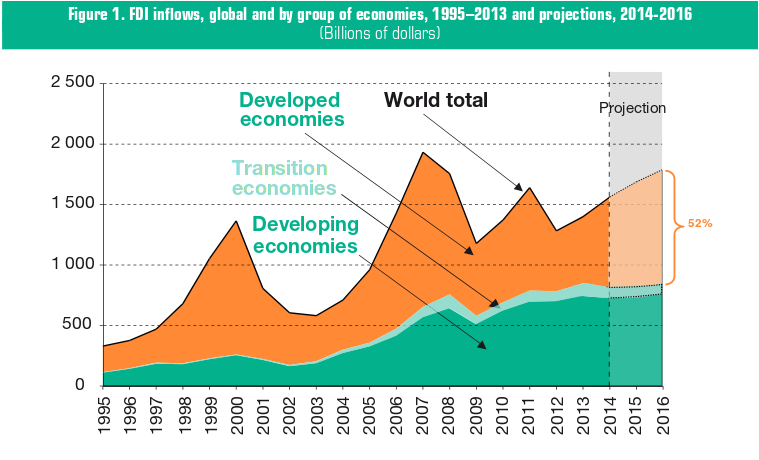
\includegraphics[width=\textwidth, height=\textheight,keepaspectratio]{../figure/global_fdi}
\caption{FDI flow to the developing economies has been increasing steadily and proves robust to economic downturn. Source: \citet[xiii]{UNCTAD2014}}
\label{fig:globalfdi}
\end{figure}

Underlying this mode of thinking is the assumption that FDI brings various benefits to developing countries, including capital and employment. However, the more important promise that FDI holds to growth is the spillover of productivity from foreign firms to domestic firms. As well-known from neoclassical growth theory, diminishing returns to capital will at one point stop capital from accumulating further, preventing long-run economic growth from being permanently driven by capital accumulation alone \citep{Solow1956}. Therefore, long-run growth ultimately requires technological innovation, which FDI can supply.

This insight implies that FDI cannot promote the host country's growth simply from the amount of capital it brings. Scholars have confirmed that FDI can only have a growth-enhancing impact if there is technological spillover from the foreign to the domestic sectors \citep{Nunnenkamp2004}. This empirical finding provides support for \citet{Findlay1978}'s groundbreaking model of FDI and growth, in which technology spillover from foreign firms shift the domestic factor-price frontier to the right, allowing more output from the same input, resulting in higher profits and higher wages (i.e. higher savings) for the domestic sector. This ultimately leads to a continually increasing domestic capital stock. In this view, FDI is welfare-enhancing, providing spillover benefits to the local firms in ways that foreign firms do not take into account in their private calculations. This provides the justification for countries' using investment incentives to rectify the undersupply of FDI, closing the gap between private and social returns. 

Despite this prevailing view about the importance of FDI in providing technological spillover, there is little conclusive evidence of FDI having a positive effect on growth \citep{Nair-Reichert2001, Carkovic2002} or poverty reduction \citep{Guerra2009} (\Cref{fig:fdipoverty}). A substantial literature has developed to explain this puzzle, concluding that the growth-enhancing and spillover effect of FDI is conditional on the absorptive capacity of local firms. Cross-nationally, scholars find that FDI is more likely to have a positive growth effect when the technological gap between the local and foreign firms is small \citep{Nunnenkamp2004} and when host countries have strong financial and institutional development \citep{Durham2004}. Similarly, absorptive capacity, measured by the level of schooling in the host economy, conditions the transfer of technology between foreign and local firms across regions in China \citep{Fu2008} and countries in Latin America \citep{Willem2004}.

\begin{figure}[!ht]
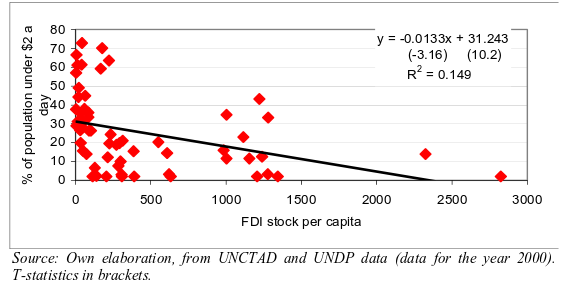
\includegraphics[width=\textwidth, height=\textheight,keepaspectratio]{../figure/fdi_poverty}
\caption{Relationship between FDI and poverty}
\label{fig:fdipoverty}
\end{figure}

Despite the resounding conclusion that the effect of FDI is highly conditional and that investment incentives do not work, why do countries still fixate so much on bringing in FDI \citep{Blomstrom2002}? For example, Ireland provided foreign investors with lower tax rate, lower land price, and cash grants for R\&D that do not need to be repaid. China also used a tax holiday (two years of no tax and three year of half the normal tax rate) in special economic zones to attract more foreign firms \citep{Telford2001}. We see the same widespread use of investment incentives in Southeast Asia \citep{Fletcher2002}. In Vietnam, the race to offer incentives to foreign firms rages on even among sub-national units, as provincial governments defied the central government's directive and offered extra-legal incentives to FDI firms \citep{Vu2007}. Not only do these measures not work in attracting more FDI, they also deprive countries of revenues that could be spent on improving the local labor quality and investment climate, which are much more conducive to spillover effect and growth.

Thus, my dissertation project focuses on this empirical puzzle: if the positive effect of FDI is uncertain, why is there so much focus on attracting it? To understand this puzzle, I propose that we need to take into account the calculus of government officials, who may be more interested in foreign firms as a source of private benefit rather than in the spillover and growth-enhancing effect of FDI. This is a potential reason why we often see countries (i.e. government officials) being so enthusiastic about attracting FDI, yet not so passionate about developing the local capacity that enables FDI to actually have a positive effect on growth.